\documentclass[11pt]{article}

\usepackage[a4paper,margin=27mm]{geometry}
\usepackage{fontspec}
\usepackage{xeCJK}
\usepackage{unicode-math}
\setmainfont{TeX Gyre Termes}
\setsansfont{TeX Gyre Heros}
\setmonofont{TeX Gyre Cursor}
\setmathfont{TeX Gyre Termes Math}
\setCJKmainfont{Noto Serif CJK SC}
\setCJKsansfont{Noto Sans CJK SC}
\setCJKmonofont{Noto Sans Mono CJK SC}

\usepackage{microtype}
\usepackage{amsthm}
\usepackage{amsmath}
\usepackage{booktabs}
\usepackage{tabularx}
\usepackage{array}
\usepackage{enumitem}
\usepackage{graphicx}
\usepackage{tikz}
\usetikzlibrary{arrows.meta,positioning,fit,calc,backgrounds}
\usepackage{placeins}
\usepackage[numbers,sort&compress]{natbib}
\usepackage{xcolor}
\usepackage{url}
\usepackage{hyperref}
\usepackage[nameinlink,noabbrev]{cleveref}

\hypersetup{
  unicode=true,
  pdftitle={Wieferich--Ulm Signatures and the Classification of Compact Arithmetic Packet Bases},
  pdfauthor={Liang Wang},
  pdfsubject={Topological classification of compact arithmetic packet bases by primary torsion-closure quotients and Ulm invariants},
  pdfkeywords={profinite abelian groups, Ulm invariants, Wieferich primes, Pontryagin duality, compact packet bases},
  colorlinks=true,
  linkcolor=blue!45!black,
  citecolor=green!35!black,
  urlcolor=blue!55!black
}

\setlength{\parindent}{1.35em}
\setlength{\parskip}{0.22em}
\setlength{\emergencystretch}{3em}
\setlist{nosep,leftmargin=2em}
\renewcommand{\arraystretch}{1.16}
\newcolumntype{Y}{>{\raggedright\arraybackslash}X}
\newcolumntype{P}[1]{>{\raggedright\arraybackslash}p{#1}}

\newtheorem{theorem}{Theorem}[section]
\newtheorem{proposition}[theorem]{Proposition}
\newtheorem{lemma}[theorem]{Lemma}
\newtheorem{corollary}[theorem]{Corollary}
\theoremstyle{definition}
\newtheorem{definition}[theorem]{Definition}
\newtheorem{remark}[theorem]{Remark}

\newcommand{\Zhat}{\widehat{\mathbf Z}}
\newcommand{\Zell}{\mathbf Z_\ell}
\newcommand{\Zr}{\mathbf Z_r}
\newcommand{\Q}{\mathbf Q}
\newcommand{\Fr}{\mathbf F_r}
\newcommand{\Up}{U_p}
\newcommand{\Hp}{H_p}
\newcommand{\Bp}{B_p}
\newcommand{\Bq}{B_q}
\newcommand{\Bpr}{B_{p,(r)}}
\newcommand{\Kpr}{K_{p,r}}
\newcommand{\PrGroup}{P_r}
\newcommand{\SrGroup}{S_r}
\newcommand{\Cyclic}[1]{C_{#1}}
\newcommand{\Pruefer}[1]{C_{#1^\infty}}
\newcommand{\TopIso}{\cong_{\mathrm{top}}}
\DeclareMathOperator{\Tor}{Tor}
\DeclareMathOperator{\Ann}{Ann}
\DeclareMathOperator{\ord}{ord}
\DeclareMathOperator{\Gal}{Gal}
\DeclareMathOperator{\res}{res}

\title{\textbf{Wieferich--Ulm Signatures and the Classification of\\
Compact Arithmetic Packet Bases}}
\author{\textbf{Liang Wang}\\
\small School of Artificial Intelligence and Automation\\
\small Huazhong University of Science and Technology (HUST)\\
\small \href{mailto:wangliang.f@gmail.com}{wangliang.f@gmail.com}}
\date{22 August 2026}

\begin{document}
\maketitle

\begin{center}
\fbox{\begin{minipage}{0.90\linewidth}
\centering
\textbf{User-authorized Stage-2 research draft.}
The underlying proof ledger has undergone internal source-domain and
devil's-advocate checks; these do not replace the separate manuscript-integrity,
release, or submission reviews.  No computational execution, Route-A/Route-B
advancement, or publication authority is claimed.
\end{minipage}}
\end{center}

\begin{abstract}
For a rational prime $p$, let
$U_p=\prod_{\ell\ne p}\mathbf Z_\ell^\times$, let
$e_p:\widehat{\mathbf Z}\to U_p$ be the continuous exponent map
$a\mapsto p^a$, and put $B_p=U_p/e_p(\widehat{\mathbf Z})$.
These compact abelian groups arise as arithmetic packet bases, but their
topological isomorphism types are not visible from the omitted coordinate
alone.  This paper computes the complete primary structure of the unmarked
groups $B_p$.  For every rational prime $r$, define
\[
\kappa_r(p)=
\begin{cases}
0,&r=p,\\
v_r(p^{r-1}-1)-1,&r\ne p\text{ and }r\text{ is odd},\\
v_2(p^2-1)-3,&r=2\text{ and }p\text{ is odd}.
\end{cases}
\]
If $B_{p,(r)}$ is the pro-$r$ Sylow factor and
$A_{p,r}=\overline{\operatorname{Tor}(B_{p,(r)})}$, then
$A_{p,r}\cong\prod_{n\ge1}(C_{r^n})^{\aleph_0}$ and
$B_{p,(r)}/A_{p,r}\cong C_{r^{\kappa_r(p)}}$.
The proof combines an exceptional-primary triangular kernel split with an
off-local exact-order Kummer--Chebotarev construction.  The latter yields
roots inside the relevant restriction kernel, not merely in an ambient
Pruefer group, and determines the full finite and transfinite Ulm sequence.
Consequently,
\[
B_p\cong_{\mathrm{top}}B_q
\quad\Longleftrightarrow\quad
\kappa_r(p)=\kappa_r(q)\ \text{for every prime }r.
\]
At $r=11$ this separates $B_2$ from $B_3$.  The theorem concerns the bare
compact quotient only: it does not recover marked coordinates, actual packet
topology, measure, flow, trace, operator, or determinant data.  Injectivity of
the full signature $p\mapsto(\kappa_r(p))_r$ is not resolved here.

\medskip
\noindent\textbf{Keywords:} profinite abelian groups; Ulm invariants;
Wieferich defects; Pontryagin duality; compact arithmetic packet bases
\end{abstract}

\begin{center}
\textbf{中文摘要}
\end{center}
\begingroup\small
\noindent
对有理素数 $p$，令
$U_p=\prod_{\ell\ne p}\mathbf Z_\ell^\times$，以连续指数映射
$e_p:\widehat{\mathbf Z}\to U_p$ 定义裸紧商群
$B_p=U_p/e_p(\widehat{\mathbf Z})$。这些群来自算术 packet 基底，但其裸拓扑
同构型不能由被删去的坐标直接读出。本文先证明 $e_p$ 为闭嵌入并建立规范主分解，
再计算 $B_p$ 的全部主分量与 Ulm 不变量。对每个素数 $r$，局部缺陷
$\kappa_r(p)$ 在 $r=p$ 时为零，在奇素数 $r\ne p$ 时为
$v_r(p^{r-1}-1)-1$，在 $r=2$、$p$ 为奇数时为 $v_2(p^2-1)-3$。
若 $A_{p,r}$ 是 $B_p$ 的 pro-$r$ 分量中扭元子群的闭包，则
$A_{p,r}\cong\prod_{n\ge1}(C_{r^n})^{\aleph_0}$，且特征商群为
$C_{r^{\kappa_r(p)}}$。对角分支不能从原始因子直接推出有界角色满射，故以
齐次三角分解和 Kulikov 吸收处理；非对角分支则在有限 Galois 复合扩张中对
Frobenius 共轭类应用 Kummer--Chebotarev 构造，同时控制素数坐标和
$p$ 的精确阶，并以有限坐标修正把各深度的根留在限制核内。这给出完整有限及
超限 Ulm 序列。最终，$B_p$ 与 $B_q$ 拓扑同构，当且仅当所有 $\kappa_r$
坐标相等；$r=11$ 已区分 $B_2$ 与 $B_3$。结论仅属于无标记裸紧群，不转移到
实际 packet、测度、流、迹、算子或行列式。证明还严格区分裸群不变量与标记、
测度及动力学对象的所有权，防止将分类结论越界转移；该签名对全部素数是否单射，
本文不作结论。

\medskip
\noindent\textbf{中文关键词：} 前有限阿贝尔群；Ulm 不变量；Wieferich 缺陷；
Pontryagin 对偶；算术 packet 基底
\endgroup

\section{Introduction and main results}\label{sec:introduction}

The compact groups studied here originate in Deninger's arithmetic-dynamical
packet construction.  In the notation used below, the source supplies the
quotient
\[
 B_p=\widehat{\mathbf Z}_{(p)}^{\times}/p^{\widehat{\mathbf Z}}
     \cong \operatorname{Aut}(\overline{\mathbf F}_p^{\times})/
             \operatorname{Aut}(\overline{\mathbf F}_p)
\]
and a choice-dependent packet fibration over it
\citep[equations~(38)--(40), Section~6, and Theorem~6.1]{Deninger2020}.
That provenance does not identify the topology of an actual packet quotient
with the compact topology of $B_p$, nor does it determine the Sylow or Ulm
structure.  The present question is therefore intrinsic and purely
topological: what information about $p$ is retained by the unmarked compact
abelian group $B_p$?

The answer is a full classification by local Wieferich depths.  The depth at
the missing primary coordinate is zero.  At an odd off-local prime $r$, it is
the excess $r$-adic valuation of $p^{r-1}-1$ beyond Fermat's forced factor.
At $r=2$, the sign and principal-unit factors must be separated, producing
$v_2(p^2-1)-3$.  These numbers are assembled into the signature
$\kappa(p)=(\kappa_r(p))_r$.

\begin{theorem}[Primary torsion-closure structure]\label{thm:primary-structure}
For every pair of rational primes $p,r$, let $B_{p,(r)}$ be the pro-$r$
Sylow factor of $B_p$ and put
\[
 A_{p,r}=\overline{\Tor(B_{p,(r)})}.
\]
Then
\begin{equation}\label{eq:factor-type}
 A_{p,r}\TopIso P_r,
 \qquad
 B_{p,(r)}/A_{p,r}\TopIso C_{r^{\kappa_r(p)}},
 \qquad
 P_r=\prod_{n\ge1}(C_{r^n})^{\aleph_0}.
\end{equation}
In particular, $\kappa_r(p)$ is intrinsic to the unmarked compact group.
\end{theorem}

\begin{theorem}[Complete classification]\label{thm:classification}
For rational primes $p$ and $q$,
\begin{equation}\label{eq:classification}
 B_p\TopIso B_q
 \quad\Longleftrightarrow\quad
 \kappa_r(p)=\kappa_r(q)
 \quad\text{for every rational prime }r.
\end{equation}
\end{theorem}

\begin{corollary}[An explicit separation]\label{cor:b2b3}
$B_2$ and $B_3$ are not topologically isomorphic.
\end{corollary}

Three transitions are load-bearing.  First, the diagonal branch $r=p$ does
not satisfy the bounded-character surjectivity that one might try to infer
from primitive divisors.  It requires a separate homogeneous triangular
split and a Kulikov subgroup argument.  Second, for $r\ne p$ the proof forces
both $v_r(\ell-1)=m$ and $v_r(\ord_\ell(p))=m$.  Divisibility of the order is
not enough.  Third, ambient Pruefer divisibility does not by itself compute
the infinite-height subgroup of the kernel; a saturated finite-coordinate
correction is needed to construct roots inside that kernel.

\begin{figure}[htbp]
\centering
\resizebox{\linewidth}{!}{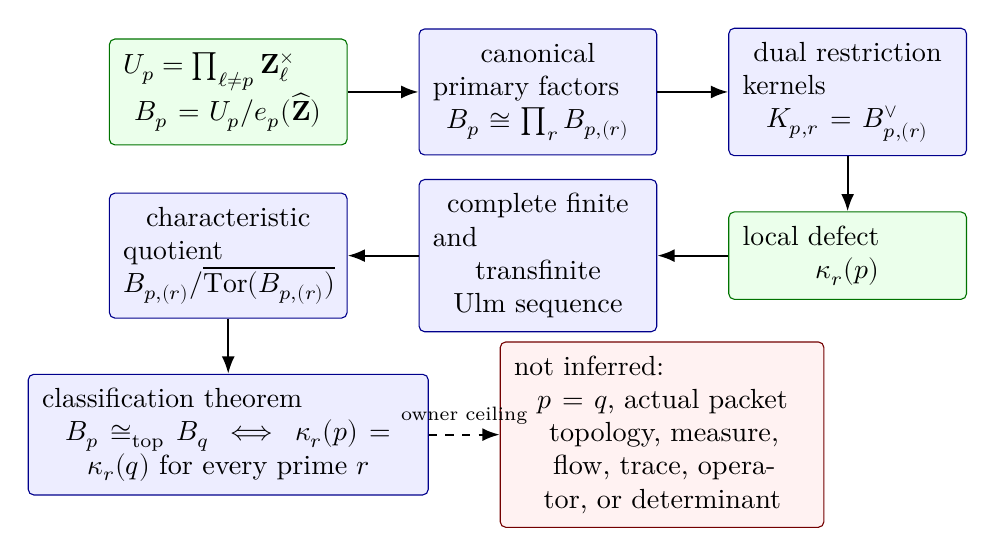
\begin{tikzpicture}[
  node distance=7mm and 9mm,
  box/.style={draw,rounded corners=2pt,align=center,inner sep=5pt,text width=0.22\linewidth},
  theorem/.style={box,fill=blue!7,draw=blue!55!black},
  arithmetic/.style={box,fill=green!8,draw=green!45!black},
  boundary/.style={box,fill=red!5,draw=red!45!black},
  arrow/.style={-{Latex[length=2.2mm]},thick},
  dashedarrow/.style={-{Latex[length=2.2mm]},thick,dashed}
]
\node[arithmetic] (owner) {$U_p=\prod_{\ell\ne p}\mathbf Z_\ell^\times$\newline
  $B_p=U_p/e_p(\widehat{\mathbf Z})$};
\node[theorem,right=of owner] (primary) {canonical primary factors\newline
  $B_p\cong\prod_r B_{p,(r)}$};
\node[theorem,right=of primary] (dual) {dual restriction kernels\newline
  $K_{p,r}=B_{p,(r)}^\vee$};

\node[arithmetic,below=of dual] (defect) {local defect\newline
  $\kappa_r(p)$};
\node[theorem,left=of defect] (ulm) {complete finite and\newline transfinite Ulm sequence};
\node[theorem,left=of ulm] (compact) {characteristic quotient\newline
  $B_{p,(r)}/\overline{\operatorname{Tor}(B_{p,(r)})}$};

\node[theorem,below=of compact,text width=0.39\linewidth] (classification) {classification theorem\newline
  $B_p\cong_{\mathrm{top}}B_q\iff
  \kappa_r(p)=\kappa_r(q)$ for every prime $r$};
\node[boundary,right=of classification,text width=0.31\linewidth] (firewall) {not inferred:\newline
  $p=q$, actual packet topology, measure, flow, trace, operator, or determinant};

\draw[arrow] (owner) -- (primary);
\draw[arrow] (primary) -- (dual);
\draw[arrow] (dual) -- (defect);
\draw[arrow] (defect) -- (ulm);
\draw[arrow] (ulm) -- (compact);
\draw[arrow] (compact) -- (classification);
\draw[dashedarrow] (classification) -- node[above,font=\scriptsize]{owner ceiling} (firewall);
\end{tikzpicture}
}
\caption{Proof architecture and owner ceiling.  Arithmetic exact-order data
enter through the restriction kernels, the complete Ulm ledger determines the
primary factor, and the unrestricted product gives the global classification.
The dashed arrow marks conclusions that are not licensed by the theorem.}
\label{fig:architecture}
\end{figure}

The local calculations also clarify the relation to the larger flow-systems
program.  Route A evaluates arithmetic dynamical systems with an intrinsic
clock, periodic-orbit structure, and a specified dynamical zeta or Fredholm
determinant.  Route B requires a Hilbert space, an operator with domain, an
exact arithmetic trace, and a completed-zeta determinant belonging to one
construction.  This paper supplies none of those objects.  The Route-A
required-input screen is therefore \texttt{NOT\_TESTABLE}; no A0--A4 tuple or
overall Route-A verdict is assigned.  Route-B advancement is not authorized, and
its exact overall status for this object is
\texttt{ROUTE\_B\_NOT\_TESTABLE}.

The paper proceeds from the compact owner and duality conventions to the
closed exponent embedding, the local restriction maps, the diagonal and
off-diagonal kernels, the full Ulm sequence, and the compact classification.
The final sections separate marked from unmarked information and state the
route, computational, and publication limits.

\section{Compact packet bases and Ulm conventions}\label{sec:preliminaries}

All compact groups are Hausdorff and all groups are abelian.  Discrete
primary groups are written additively.  For a prime $r$, write $C_{r^n}$ for
the cyclic group of order $r^n$, set $C_{r^0}=1$, and write
$C_{r^\infty}$ for the Pruefer $r$-group.  Pontryagin duals are denoted by
$G^\vee$.

For a rational prime $p$, define
\begin{equation}\label{eq:owner}
 U_p=\prod_{\ell\ne p}\mathbf Z_\ell^\times,
 \qquad
 e_p:\widehat{\mathbf Z}\longrightarrow U_p,
 \quad a\longmapsto p^a,
\end{equation}
and put
\begin{equation}\label{eq:quotient}
 H_p=e_p(\widehat{\mathbf Z}),
 \qquad
 B_p=U_p/H_p.
\end{equation}
The meaning of $p^a$ is coordinatewise: the ordinary map
$n\mapsto p^n$ from $\mathbf Z$ to each $\mathbf Z_\ell^\times$ extends
continuously to $\widehat{\mathbf Z}$.  The continuity and injectivity of the
product map are proved in \cref{sec:embedding}.

\begin{lemma}[Exact dual sequence]\label{lem:dual-sequence}
If $H$ is a closed subgroup of an abelian profinite group $G$, restriction
gives an exact sequence of discrete groups
\begin{equation}\label{eq:dual-sequence}
0\longrightarrow (G/H)^\vee\longrightarrow G^\vee
\longrightarrow H^\vee\longrightarrow0.
\end{equation}
For a closed subgroup $A\le G$,
\begin{equation}\label{eq:annihilator-duality}
A^\vee\cong G^\vee/A^\perp,
\qquad
(G/A)^\vee\cong A^\perp.
\end{equation}
\end{lemma}

\begin{proof}
A character of $G/H$ pulls back precisely to a character of $G$ that
annihilates $H$.  For surjectivity of restriction, let
$\chi:H\to\mathbf R/\mathbf Z$ be continuous.  Its image is finite in the
profinite setting, and its kernel is open.  Choose an open subgroup $V\le G$
with $V\cap H\subseteq\ker\chi$.  The character then factors through the
subgroup $H/(V\cap H)$ of the finite abelian group $G/V$.  Characters of
subgroups of finite abelian groups extend to the ambient finite group, for
example by cyclic primary decomposition and divisibility of
$\mathbf R/\mathbf Z$.  Pulling an extension back to $G$ proves surjectivity.
The annihilator identities follow from the same correspondence.
\end{proof}

\begin{lemma}[Canonical primary factors]\label{lem:primary-decomposition}
Every abelian profinite group has a canonical unrestricted product
decomposition
\begin{equation}\label{eq:primary-decomposition}
G\TopIso\prod_rG_{(r)},
\end{equation}
where $G_{(r)}$ is the unique pro-$r$ Sylow factor.  Each factor is
characteristic, and closed subgroups and quotients respect the decomposition.
\end{lemma}

\begin{proof}
Every finite abelian quotient is canonically the product of its primary
Sylow subgroups, compatibly with transition maps.  Taking the inverse limit
gives \eqref{eq:primary-decomposition}.  Uniqueness implies characteristicity.
The primary idempotents in finite quotients restrict to a closed subgroup and
descend through a compact quotient map.
\end{proof}

Define
\begin{equation}\label{eq:PS}
P_r=\prod_{n\ge1}(C_{r^n})^{\aleph_0},
\qquad
S_r=P_r^\vee=\bigoplus_{n\ge1}(C_{r^n})^{(\aleph_0)}.
\end{equation}
For a discrete $r$-group $K$, use the transfinite filtration
\begin{equation}\label{eq:transfinite-filtration}
r^0K=K,
\qquad r^{\alpha+1}K=r(r^\alpha K),
\qquad r^\lambda K=\bigcap_{\alpha<\lambda}r^\alpha K
\end{equation}
at a limit ordinal $\lambda$.  In particular,
$r^\omega K=\bigcap_{m\ge0}r^mK$.  With
$J[r]=\{x\in J:rx=0\}$, the Ulm invariant at an ordinal $\alpha$ is
\begin{equation}\label{eq:ulm}
u_\alpha(K)=\dim_{\mathbf F_r}
\frac{(r^\alpha K)[r]}{(r^{\alpha+1}K)[r]}.
\end{equation}
The final classification uses Kiehlmann's countably based dual-reduced
theorem only after countability, reducedness, and the complete sequence in
\eqref{eq:ulm} have been established
\citep[Definition~1.3, Theorems~1.4 and~1.8]{Kiehlmann2013}.

\section{The exponent embedding and ambient primary factors}\label{sec:embedding}

\begin{proposition}[Closed exponent embedding]\label{prop:embedding}
The map $e_p$ in \eqref{eq:owner} is a continuous injection and hence a
homeomorphism from $\widehat{\mathbf Z}$ onto the closed subgroup $H_p$.
\end{proposition}

\begin{proof}
For $\ell\ne p$, the map $\mathbf Z\to\mathbf Z_\ell^\times$,
$n\mapsto p^n$, is continuous for the profinite topology: the inverse image
of an open subgroup contains $d\mathbf Z$, where $d$ is the order of $p$ in
the associated finite quotient.  It therefore extends uniquely to
$\widehat{\mathbf Z}$.  Taking the product proves continuity.

Write $\widehat{\mathbf Z}=\prod_r\mathbf Z_r$ and examine the pro-$r$
factor.  If $r\ne p$ is odd, use the decomposition
\[
p=\omega_r(p)\langle p\rangle_r,
\qquad
\omega_r(p)\in\mu_{r-1},
\quad \langle p\rangle_r\in1+r\mathbf Z_r.
\]
The pro-$r$ exponent kills the prime-to-$r$ Teichmueller factor and acts on
principal units through multiplication by the nonzero element
$\log\langle p\rangle_r$.  The logarithm
$1+r\mathbf Z_r\to r\mathbf Z_r$ is an isomorphism in the required domain
\citep[Example~8.15]{ConradInfiniteSeries}.  Since $\mathbf Z_r$ is an
integral domain, the kernel is zero.  If $r=2\ne p$, choose
$\epsilon_p\in\{\pm1\}$ with $u_p=\epsilon_pp\in1+4\mathbf Z_2$ and apply
the logarithm on $1+4\mathbf Z_2$; the principal unit is again nontrivial
\citep[Theorem~2.6 and Remark~2.8]{ConradPadicInterpolation}.

The missing coordinate $r=p$ needs a different detector.  For each $m\ge1$,
apply the Bang--Zsigmondy theorem to $p^{p^m}-1$.  Its three classical
exceptions do not occur: the exponent is not $1$; when it is $2$, one has
$p=2$, $m=1$, and $p+1=3$, not a power of $2$; and $6$ is not a prime
power.  A primitive divisor $\ell\ne p$ therefore satisfies
\begin{equation}\label{eq:zsigmondy-order}
\ord_\ell(p)=p^m.
\end{equation}
This is exactly the original theorem's primitive-divisor use, sharpened to
its printed theorem page
\citep[p.~283]{Zsigmondy1892}.  If $p^a=1$ in every away coordinate, then
\eqref{eq:zsigmondy-order} forces the $\mathbf Z_p$ component of $a$ to
vanish modulo every $p^m$.  All primary components of $a$ are thus zero.
Compactness of $\widehat{\mathbf Z}$ and Hausdorffness of $U_p$ make the
image closed.
\end{proof}

\begin{proposition}[Ambient primary factors]\label{prop:ambient-factors}
For every prime $r$,
\begin{equation}\label{eq:ambient-factors}
U_{p,(r)}\TopIso
\begin{cases}
P_r,&r=p,\\
\mathbf Z_r\times P_r,&r\ne p.
\end{cases}
\end{equation}
Consequently,
\begin{equation}\label{eq:B-primary}
B_p\TopIso\prod_rB_{p,(r)},
\qquad
B_{p,(r)}=U_{p,(r)}/e_p(\mathbf Z_r),
\end{equation}
and all displayed compact groups are countably based.
\end{proposition}

\begin{proof}
For an odd prime $\ell\ne r$, the pro-$r$ Sylow subgroup of
$\mathbf Z_\ell^\times$ is cyclic of order $r^{v_r(\ell-1)}$.  For each
$n\ge1$, Dirichlet's theorem applied to the reduced residue class
$1+r^n\pmod{r^{n+1}}$ supplies infinitely many primes $\ell$ with
\begin{equation}\label{eq:dirichlet-valuation}
v_r(\ell-1)=n
\end{equation}
\citep[Theorem~18.1]{Sutherland2021Dirichlet}.
After the finitely many forbidden coordinates are removed, each finite cyclic
order still occurs countably infinitely often.  The local coordinate
$\ell=r$, when present, contributes $\mathbf Z_r$ for odd $r$ and
\begin{equation}\label{eq:two-units}
\mathbf Z_2^\times\cong C_2\times\mathbf Z_2
\end{equation}
for $r=2$.  In the latter case the finite $C_2$ is abstractly absorbed into
the already countable family of order-$2$ factors; its restriction-map
contribution will be retained in \cref{sec:restriction}.  The local coordinate
is absent precisely when $r=p$, proving \eqref{eq:ambient-factors}.  Apply
\cref{lem:primary-decomposition} to the closed subgroup $H_p$ and its quotient
to obtain \eqref{eq:B-primary}.  Countability of the coordinate set gives a
countable base.
\end{proof}

\section{Restriction maps and the local Wieferich defect}\label{sec:restriction}

Put
\begin{equation}\label{eq:K-definition}
K_{p,r}=B_{p,(r)}^\vee.
\end{equation}
Applying \cref{lem:dual-sequence} to \eqref{eq:B-primary} gives
\begin{equation}\label{eq:restriction}
0\longrightarrow K_{p,r}\longrightarrow U_{p,(r)}^\vee
\xrightarrow{\res_{p,r}} C_{r^\infty}\longrightarrow0.
\end{equation}
The arrows matter: surjectivity is extension of a continuous character from
the closed subgroup $e_p(\mathbf Z_r)$, not a claim that every bounded-order
character extends with the same order.

When $r=p$, \eqref{eq:restriction} has the form
\begin{equation}\label{eq:diagonal-map}
0\longrightarrow K_{p,p}\longrightarrow S_p
\xrightarrow{g_p}C_{p^\infty}\longrightarrow0.
\end{equation}
For $r\ne p$ it becomes
\begin{equation}\label{eq:off-local-map}
0\longrightarrow K_{p,r}\longrightarrow S_r\oplus C_{r^\infty}
\xrightarrow{\Phi_{p,r}}C_{r^\infty}\longrightarrow0.
\end{equation}

\begin{definition}[Wieferich--Ulm defect]\label{def:kappa}
For primes $p,r$, define
\begin{equation}\label{eq:kappa}
\kappa_r(p)=
\begin{cases}
0,&r=p,\\[2pt]
v_r(p^{r-1}-1)-1,&r\ne p\text{ and }r\text{ is odd},\\[2pt]
v_2(p^2-1)-3,&r=2\text{ and }p\text{ is odd}.
\end{cases}
\end{equation}
\end{definition}

\begin{proposition}[Normalized off-local map]\label{prop:normalized-map}
For $r\ne p$, automorphisms of the local source and target normalize
\eqref{eq:off-local-map} to
\begin{equation}\label{eq:normalized-map}
\Phi(s,z)=g(s)+r^{\kappa_r(p)}z,
\qquad
S_r\oplus C_{r^\infty}\longrightarrow C_{r^\infty}.
\end{equation}
\end{proposition}

\begin{proof}
Suppose first that $r$ is odd.  Since
$\langle p\rangle_r^{r-1}=p^{r-1}$ and $r-1$ is an $r$-adic unit,
the exact logarithmic valuation is
\[
v_r(\log\langle p\rangle_r)=v_r(p^{r-1}-1).
\]
Normalize $1+r\mathbf Z_r$ by a logarithmic generator of valuation $1$.
The primal map on $\mathbf Z_r$ is multiplication by an element of valuation
$\kappa_r(p)$, so its Pontryagin dual on $C_{r^\infty}$ is multiplication by
$r^{\kappa_r(p)}$ up to a unit.

For $r=2$ and $p$ odd, normalize the principal units by $\log 5$.  With
$u_p=\epsilon_pp\in1+4\mathbf Z_2$,
\begin{equation}\label{eq:two-kappa}
v_2\!\left(\frac{\log u_p}{\log5}\right)
=v_2(u_p-1)-2
=v_2(p^2-1)-3.
\end{equation}
If $p\equiv3\pmod4$, the nontrivial sign character in the literal local dual
$C_2\oplus C_{2^\infty}$ restricts to the unique order-$2$ target element;
if $p\equiv1\pmod4$, it restricts trivially.  That contribution is placed in
$g$ before the abstract $C_2$ is absorbed into $S_2$.  Only the principal
Pruefer factor is normalized as multiplication by $2^{\kappa_2(p)}$.
\end{proof}

\section{The exceptional primary branch}\label{sec:diagonal}

The case $r=p$ is algebraic and does not use off-local exact-order saturation.
The distinction is necessary even when $p=2$.

\begin{lemma}[Homogeneous triangular split]\label{lem:triangular}
Let
\[
S=\bigoplus_{n\ge1}S_n,
\qquad S_n=(C_{p^n})^{(\aleph_0)},
\qquad g:S\longrightarrow C_{p^\infty}
\]
be a homomorphism.  Then
\begin{equation}\label{eq:triangular-split}
S=T\oplus R,
\qquad T\cong S,
\qquad R\cong\bigoplus_{n\ge1}C_{p^n},
\qquad g(T)=0.
\end{equation}
Moreover,
\begin{equation}\label{eq:kernel-split}
\ker g=T\oplus\ker(g|_R)\cong S.
\end{equation}
\end{lemma}

\begin{proof}
Fix a basis $(e_{n,j})_{j\ge0}$ of each $S_n$.  Choose $e_{n,0}$ with image
of maximal order.  Subgroups of $C_{p^\infty}[p^n]$ are linearly ordered, so
$g(e_{n,0})$ generates $g(S_n)$.  For $j>0$, choose
$c_{n,j}\in\mathbf Z/p^n\mathbf Z$ and set
\[
g(e_{n,j})=c_{n,j}g(e_{n,0}),
\qquad
e'_{n,j}=e_{n,j}-c_{n,j}e_{n,0}.
\]
This is a triangular change of basis on the algebraic direct sum.  The
$e'_{n,j}$ have exact order $p^n$ and lie in the kernel.  Thus
$S_n=T_n\oplus R_n$ with
$T_n\cong(C_{p^n})^{(\aleph_0)}$, $R_n\cong C_{p^n}$, and $g(T_n)=0$.
Taking direct sums gives \eqref{eq:triangular-split} and the literal equality
in \eqref{eq:kernel-split}.  The subgroup $\ker(g|_R)$ of a direct sum of
cyclic primary groups is itself a direct sum of cyclic groups by Kulikov's
theorem \citep[Corollary~2, pp.~66--67]{Hill1972}.  It is countable, so each
of its cyclic multiplicities is at most $\aleph_0$ and is absorbed by the
already $\aleph_0$ copies of every order in $T$.
\end{proof}

\begin{theorem}[Diagonal Ulm ledger]\label{thm:diagonal-ledger}
For every prime $p$,
\begin{equation}\label{eq:diagonal-K}
K_{p,p}\cong S_p,
\qquad p^\omega K_{p,p}=0,
\end{equation}
and
\begin{equation}\label{eq:diagonal-ulm}
u_n(K_{p,p})=\aleph_0\quad(n<\omega),
\qquad
u_\alpha(K_{p,p})=0\quad(\alpha\ge\omega).
\end{equation}
Consequently,
\begin{equation}\label{eq:diagonal-compact}
B_{p,(p)}\TopIso P_p,
\qquad
\overline{\Tor(B_{p,(p)})}=B_{p,(p)},
\qquad
\kappa_p(p)=0.
\end{equation}
\end{theorem}

\begin{proof}
Apply \cref{lem:triangular} to the epimorphism $g_p$ in
\eqref{eq:diagonal-map}.  Every element of $S_p$ has finite support, hence no
nonzero element lies in $p^mS_p$ for every $m$.  This proves the
infinite-height assertion.  The countably many copies of $C_{p^{n+1}}$ give
the finite invariants.  Pontryagin duality yields
\eqref{eq:diagonal-compact}; finite-support torsion points are dense in $P_p$.
\end{proof}

\begin{remark}[Withdrawn bounded-character route]\label{rem:withdrawn}
Surjectivity of \eqref{eq:restriction} does not imply
$g_p(S_p[p^m])=C_{p^\infty}[p^m]$.  For example,
$\ord_{17}(2)=8$ while $v_2(17-1)=4$, so a faithful character of the
order-$8$ subgroup of $C_{16}$ may need an extension of order $16$.
Furthermore, if $\ell\equiv1\pmod8$, then quadratic reciprocity makes $2$ a
square modulo $\ell$; one cannot require
$v_2(\ord_\ell(2))=v_2(\ell-1)\ge3$.  Thus $p=r=2$ belongs only to
\cref{thm:diagonal-ledger}.
\end{remark}

\section{Exact-order saturation off the diagonal}\label{sec:saturation}

Fix $r\ne p$ and let $g:S_r\to C_{r^\infty}$ be the away-coordinate and
sign part of \eqref{eq:normalized-map}.

\begin{lemma}[One exact coordinate]\label{lem:one-coordinate}
If a prime $\ell\ne p,r$ satisfies
\begin{equation}\label{eq:double-valuation-coordinate}
v_r(\ell-1)=m,
\qquad
v_r(\ord_\ell(p))=m,
\end{equation}
then
\begin{equation}\label{eq:coordinate-saturation}
g(S_r[r^m])=C_{r^\infty}[r^m].
\end{equation}
\end{lemma}

\begin{proof}
The pro-$r$ Sylow of $\mathbf F_\ell^\times$ is $C_{r^m}$, and the exponent
map from $\mathbf Z_r$ onto that coordinate is surjective because the
$r$-primary part of $p$ has exact order $r^m$.  Dual restriction therefore
embeds the coordinate dual onto $C_{r^\infty}[r^m]$.  The reverse inclusion
is automatic for a homomorphism on $r^m$-torsion.
\end{proof}

\begin{lemma}[Exact-order primes]\label{lem:exact-order-primes}
For every $r\ne p$ and every $m\ge1$, there are infinitely many primes
$\ell\ne p,r$ satisfying \eqref{eq:double-valuation-coordinate}.
\end{lemma}

\begin{proof}
Assume first that $r$ is odd.  Set
\[
F=\mathbf Q(\zeta_r),
\qquad L=F(p^{1/r}),
\qquad C_m=\mathbf Q(\zeta_{r^{m+1}}).
\]
The polynomial $X^r-p$ is Eisenstein at every prime of $F$ above $p$, so
$L/F$ is a nontrivial cyclic Kummer extension of degree $r$ ramified above
$p$.  The cyclotomic extension $C_m/F$ is ramified only above $r$.
Consequently,
\begin{equation}\label{eq:odd-intersection}
L\cap C_m=F.
\end{equation}
Choose an automorphism of $C_m/F$ sending
$\zeta_{r^{m+1}}$ to $\zeta_{r^{m+1}}^{1+r^m}$ and a nontrivial Kummer
automorphism sending $p^{1/r}$ to $\zeta_rp^{1/r}$.  Equation
\eqref{eq:odd-intersection} makes them compatible in the compositum
$E=LC_m$, defining an element $\sigma\in\Gal(E/F)$.  The field $L$ is the
splitting field of $X^r-p$ over $\mathbf Q$, so $E/\mathbf Q$ is finite
Galois.  Apply the qualitative Chebotarev theorem to the conjugacy class of
$\sigma$ in $\Gal(E/\mathbf Q)$.  Every conjugate still fixes $F$; its
restriction to $C_m$ is unchanged because $\Gal(C_m/\mathbf Q)$ is abelian,
and its restriction to $L$ is a nonidentity element of $\Gal(L/F)$.  Hence there are infinitely
many unramified rational primes with this Frobenius class
\citep[Theorem~28.9]{Sutherland2021Chebotarev}; the stable historical
source is \citet{LagariasOdlyzko1977}.  Such a prime splits completely in
$F$, so the relevant residue field is $\mathbf F_\ell$.  Its cyclotomic
component yields $v_r(\ell-1)=m$, while the nontrivial Kummer component says
that $p$ is not an $r$th power in $\mathbf F_\ell^\times$.  In a cyclic group
whose order has $r$-valuation $m$, that is equivalent to
$v_r(\ord_\ell(p))=m$.

For $r=2$, the prime $p$ is odd.  Put
$L=\mathbf Q(\sqrt p)$ and $C_m=\mathbf Q(\zeta_{2^{m+1}})$.  The first
field is ramified at the odd prime $p$ and the second only at $2$, so
$L\cap C_m=\mathbf Q$.  Combine the nontrivial quadratic automorphism with
the cyclotomic exponent $1+2^m$.  The compositum $LC_m/\mathbf Q$ is finite
abelian, so Chebotarev applies directly to this combined element and gives
infinitely many primes with
\[
v_2(\ell-1)=m,
\qquad
\left(\frac p\ell\right)=-1.
\]
Nonsquareness in the cyclic group $\mathbf F_\ell^\times$ is equivalent to
$v_2(\ord_\ell(p))=m$.  The argument includes $m=1$ and is disjoint from the
diagonal $p=r=2$ case.
\end{proof}

\begin{theorem}[Bounded restriction saturation]\label{thm:saturation}
For every $r\ne p$ and every $m\ge1$,
\begin{equation}\label{eq:saturation}
g(S_r[r^m])=C_{r^\infty}[r^m].
\end{equation}
\end{theorem}

\begin{proof}
Combine \cref{lem:one-coordinate,lem:exact-order-primes}.  The theorem is
unconditional and qualitative; it uses neither GRH nor an effective density
estimate.  Moree's results on divisibility of multiplicative orders form a
close comparator but do
not supply the simultaneous equalities in
\eqref{eq:double-valuation-coordinate} \citep{Moree2005}.
\end{proof}

\section{Kernel-internal roots and the complete Ulm sequence}\label{sec:ulm}

For $r\ne p$, write $\kappa=\kappa_r(p)$ and
\begin{equation}\label{eq:kernel}
K=K_{p,r}=\ker\Phi,
\qquad
\Phi(s,z)=g(s)+r^\kappa z.
\end{equation}
Applying the triangular construction to $g:S_r\to C_{r^\infty}$ yields
\begin{equation}\label{eq:killed-summand}
S_r=T\oplus R,
\qquad T\cong S_r,
\qquad g(T)=0,
\end{equation}
and hence an internal split
\begin{equation}\label{eq:K-split}
K=T\oplus K^0,
\qquad
K^0=\ker\bigl(\Phi|_{R\oplus C_{r^\infty}}\bigr).
\end{equation}
This homogeneous summand supplies the finite multiplicities; the next
theorem computes infinite height.

\begin{theorem}[Infinite-height subgroup]\label{thm:infinite-height}
Inside $S_r\oplus C_{r^\infty}$,
\begin{equation}\label{eq:infinite-height}
r^\omega K_{p,r}=0\oplus C_{r^{\kappa_r(p)}}.
\end{equation}
\end{theorem}

\begin{proof}
If $(s,z)$ lies in $r^mK$ for every $m$, then $s$ belongs to
$\bigcap_mr^mS_r=0$.  The kernel equation then gives $r^\kappa z=0$,
which proves the upper inclusion in \eqref{eq:infinite-height}.

For the reverse inclusion, take $z\in C_{r^\infty}[r^\kappa]$ and fix
$m\ge1$.  Choose an ambient Pruefer root $w_m$ with $r^mw_m=z$.  Then
$r^\kappa w_m\in C_{r^\infty}[r^m]$.  By \cref{thm:saturation}, choose
$s_m\in S_r[r^m]$ satisfying
\begin{equation}\label{eq:kernel-correction}
g(s_m)=-r^\kappa w_m.
\end{equation}
Thus $(s_m,w_m)$ lies in $K$ and
$r^m(s_m,w_m)=(0,z)$.  The root is now inside the kernel.  Since this works
for every $m$, $(0,z)\in r^\omega K$.
\end{proof}

\begin{proposition}[Complete Ulm ledger]\label{prop:ulm-ledger}
For every $r\ne p$,
\begin{equation}\label{eq:finite-ulm}
u_n(K_{p,r})=\aleph_0\qquad(n<\omega).
\end{equation}
If $\kappa_r(p)>0$, then
\begin{equation}\label{eq:transfinite-ulm}
u_{\omega+\kappa_r(p)-1}(K_{p,r})=1
\end{equation}
and every other invariant at an ordinal $\alpha\ge\omega$ is zero.  If
$\kappa_r(p)=0$, every invariant at $\alpha\ge\omega$ is zero.  In all
cases $K_{p,r}$ is countable and reduced.
\end{proposition}

\begin{proof}
The summand $T\cong S_r$ in \eqref{eq:K-split} contains countably many copies
of $C_{r^{n+1}}$ for every $n$, giving the lower bound in
\eqref{eq:finite-ulm}.  The entire ambient group is countable, which gives
equality.  If $\kappa>0$, \cref{thm:infinite-height} yields
\[
r^{\omega+j}K=r^jC_{r^\kappa}\cong C_{r^{\kappa-j}}
\quad(0\le j\le\kappa),
\qquad
r^{\omega+\kappa}K=0.
\]
The order-$r$ subgroups of consecutive terms agree until the last nonzero
step, where the quotient is $C_r$.  This gives
\eqref{eq:transfinite-ulm}; the case $\kappa=0$ is immediate.  Finally, a
divisible subgroup of $K$ must lie in $r^\omega K$, which is finite.  A
finite divisible group is zero, so $K$ is reduced.
\end{proof}

\section{Torsion closure and primary compact structure}\label{sec:compact}

\begin{lemma}[Torsion-closure annihilator]\label{lem:torsion-annihilator}
Let $K$ be a discrete $r$-group and $B=K^\vee$.  Then
\begin{equation}\label{eq:torsion-annihilator}
\Ann\bigl(\overline{\Tor(B)}\bigr)=r^\omega K.
\end{equation}
\end{lemma}

\begin{proof}
If $x\in r^\omega K$ and $\chi\in B$ has order dividing $r^m$, write
$x=r^my$; then $\chi(x)=0$.  Thus $r^\omega K$ annihilates torsion and its
closure.  Conversely, if $x\notin r^\omega K$, choose $m$ with
$x\notin r^mK$.  A character of the bounded quotient $K/r^mK$ separates the
nonzero class of $x$, and it pulls back to a finite-order point of $B$ that
does not annihilate $x$.  This is the direct form of Kiehlmann's
torsion-closure/infinite-height correspondence
\citep[Theorem~1.1]{Kiehlmann2013}.
\end{proof}

\begin{proof}[Proof of \cref{thm:primary-structure}]
The diagonal case is \cref{thm:diagonal-ledger}, so suppose $r\ne p$.  Put
$N=r^\omega K_{p,r}$.  By \cref{lem:torsion-annihilator} and Pontryagin
duality,
\begin{equation}\label{eq:compact-duals}
A_{p,r}^\vee\cong K_{p,r}/N,
\qquad
(B_{p,(r)}/A_{p,r})^\vee\cong N.
\end{equation}
Projection onto the $S_r$ coordinate gives an exact sequence
\begin{equation}\label{eq:projection-exact}
0\longrightarrow N\longrightarrow K_{p,r}
\xrightarrow{\pi_S}S_r\longrightarrow0.
\end{equation}
Indeed, multiplication by $r^\kappa$ on $C_{r^\infty}$ is surjective, so
for every $s\in S_r$ there is $z$ with $r^\kappa z=-g(s)$; the kernel of
$\pi_S$ is precisely $0\oplus C_{r^\kappa}=N$.  Hence
$K_{p,r}/N\cong S_r$.  Dualizing and using
\cref{thm:infinite-height} in \eqref{eq:compact-duals} yields
\[
A_{p,r}\TopIso P_r,
\qquad
B_{p,(r)}/A_{p,r}\TopIso C_{r^\kappa}.
\]
\end{proof}

Because $B_{p,(r)}$ is characteristic and the closure of its torsion is
characteristic, \cref{thm:primary-structure} gives the intrinsic formula
\begin{equation}\label{eq:intrinsic-kappa}
\kappa_r(p)=
\log_r\bigl[B_{p,(r)}:\overline{\Tor(B_{p,(r)})}\bigr].
\end{equation}
No coordinate label of $U_p$ appears in \eqref{eq:intrinsic-kappa}.

\section{Global classification and arithmetic separation}\label{sec:classification}

\begin{proof}[Proof of \cref{thm:classification}]
Suppose $B_p\TopIso B_q$.  A topological isomorphism carries the unique
characteristic pro-$r$ factor onto the pro-$r$ factor and carries the closure
of torsion onto the closure of torsion.  The indices in
\eqref{eq:intrinsic-kappa} therefore agree for every $r$, proving necessity.

Conversely, suppose $\kappa_r(p)=\kappa_r(q)$ for all $r$.  The discrete
duals $K_{p,r}$ and $K_{q,r}$ are countable and reduced.  Their finite Ulm
invariants are all $\aleph_0$, and their complete transfinite invariants
agree by \cref{thm:diagonal-ledger,prop:ulm-ledger}.  Kiehlmann identifies
these full Ulm sequences with the compact torsion sequences and classifies
countably based dual-reduced pro-$r$ groups by that complete data
\citep[Remark~1.6 and Theorem~1.8]{Kiehlmann2013}.  Hence
$K_{p,r}\cong K_{q,r}$, and duality gives a homeomorphism
$\varphi_r:B_{p,(r)}\to B_{q,(r)}$.  The unrestricted product
\[
\prod_r\varphi_r:
\prod_rB_{p,(r)}\longrightarrow\prod_rB_{q,(r)}
\]
is a homeomorphism with inverse $\prod_r\varphi_r^{-1}$.  Apply
\eqref{eq:B-primary} to finish the proof.
\end{proof}

\begin{proof}[Proof of \cref{cor:b2b3}]
At $r=11$,
\[
2^{10}-1=1023=3\cdot11\cdot31,
\qquad
\kappa_{11}(2)=0,
\]
whereas
\[
3^{10}-1=59048=8\cdot11^2\cdot61,
\qquad
\kappa_{11}(3)=1.
\]
Thus
\[
B_{2,(11)}/\overline{\Tor(B_{2,(11)})}=1,
\qquad
B_{3,(11)}/\overline{\Tor(B_{3,(11)})}\cong C_{11}.
\]
These characteristic quotients cannot be carried to each other by an
isomorphism.
\end{proof}

The example is intrinsic, but it does not prove that the full signature
recovers every prime.  The classification theorem identifies isomorphism
classes with equality classes of $p\mapsto\kappa(p)$.  Injectivity of that
map is not resolved by the present argument.

\section{Marked data, prior subtraction, and theorem scope}\label{sec:scope}

The quotient theorem is deliberately unmarked.  In the presentation
\[
H_p\longrightarrow U_p\longrightarrow B_p,
\]
the dual kernels inherit finite-coordinate supports and conductor bounds.
These data are natural for the marked sequence but are not characteristic on
the bare group.  In every homogeneous block, the triangular construction
produces a summand $(C_{r^n})^{(\aleph_0)}$ in the kernel.  Basis vectors
coming from different away coordinates can be exchanged by an automorphism
while the complement is fixed.  Such an automorphism moves the marked
support filtration.  Pontryagin duality transports it to a bare compact-group
automorphism.

The ambient group $U_p$ does retain a simpler marker:
\begin{equation}\label{eq:ambient-marker}
U_{p,(r)}^\vee\text{ has a divisible }C_{r^\infty}
\quad\Longleftrightarrow\quad r\ne p.
\end{equation}
Equation \eqref{eq:ambient-marker} detects the omitted coordinate of $U_p$,
not an invariant of the quotient $B_p$.  Quotienting by $H_p$ replaces that
marker with the complete $\kappa$-ledger.

\begin{table}[htbp]
\centering\small
\caption{Source-owned input, proof-owned bridge, and retained ceiling.}
\label{tab:source-ceilings}
\begin{tabularx}{\linewidth}{P{0.22\linewidth}YY}
\toprule
Input & Used for & Not supplied by the source \\
\midrule
Deninger \citep{Deninger2020} & compact quotient provenance & packet topology, Sylow/Ulm calculation, or classification \\
Kiehlmann \citep{Kiehlmann2013} & torsion closure and final dual-reduced classification & arithmetic kernel, heights, or reduction to one defect \\
Hill/Kulikov \citep{Hill1972} & cyclic decomposition of the diagonal residual subgroup & multiplicities or packet identification \\
Zsigmondy \citep{Zsigmondy1892} & omitted-coordinate detection & bounded-character saturation \\
Dirichlet and Chebotarev \citep{Sutherland2021Dirichlet,Sutherland2021Chebotarev,LagariasOdlyzko1977} & exact congruence classes and Frobenius occurrence & the two intersections, selected automorphisms, or kernel roots \\
Conrad \citep{ConradInfiniteSeries,ConradPadicInterpolation} & logarithm domains, valuations, and the $2$-sign split & restriction saturation or Ulm conclusions \\
Moree \citep{Moree2005} & nearest multiplicative-order-divisibility comparator & simultaneous exact double valuation or compact classification \\
\bottomrule
\end{tabularx}
\end{table}

The proof-owned delta lies in the joined chain rather than in any classical
ingredient.  The diagonal restriction kernel needs a different mechanism
from the off-local one.  Off the diagonal, exact Frobenius conditions produce
bounded saturation, bounded saturation produces roots internal to the
kernel, and those roots place the arithmetic depth at the ordinal
$\omega+\kappa_r(p)-1$.  Only then is the compact classification theorem in
the domain of the standard Ulm result.

\subsection{Owner firewall}

\begin{table}[htbp]
\centering\small
\caption{Statements licensed and excluded by owner.}
\label{tab:owner-firewall}
\begin{tabularx}{\linewidth}{P{0.25\linewidth}YY}
\toprule
Owner & Licensed statement & Excluded transfer \\
\midrule
Marked $H_p\to U_p\to B_p$ & coordinate support and exponent restriction map & treating labels or conductor bounds as bare invariants \\
Bare compact group $B_p$ & \cref{thm:primary-structure,thm:classification,cor:b2b3} & importing the missing-coordinate marker \\
Actual packet quotient & no theorem in this paper & compact topology, separation, or $B_2/B_3$ transfer \\
Measured enhancement & none & Haar descent or canonical packet measure \\
Flow/time owner & none & a clock, orbit, or return theorem \\
Trace/operator/determinant & none & spectrum, explicit formula, determinant, or Route-B credit \\
\bottomrule
\end{tabularx}
\end{table}

\subsection{Internal Route-A and Route-B placement}

This is a nonnormative governance check against the local project protocols
\texttt{skills/route-a-evaluator.md} and
\texttt{skills/route-b-evaluator.md}, both version 0.2.0 in the accompanying
snapshot.  The labels below are not external scientific claims and award no
Route credit.

The repository's Route-A evaluator asks for a frozen dynamical candidate,
arithmetic origin, phase space, dynamics, clock, normalization, determinant
convention, and data split before it assigns coordinates A0--A4.  The object
defined in \eqref{eq:owner} has arithmetic provenance but no dynamics, clock,
orbit ledger, transfer operator, or determinant.  No Route-A coordinate is
therefore asserted.

Route B is a proof route that requires the arithmetic, periodic-orbit,
operator, trace, and determinant sides to belong to the same mathematical
object.  Its minimum input includes an explicit Hilbert space, inner product,
dense domain, boundary conditions, operator action, clock, and normalization.
None appears in this paper.  Accordingly, Route-B advancement is not authorized,
the construction is \texttt{ROUTE\_B\_NOT\_TESTABLE}, and no
Hilbert--Polya claim is allowed.

\section{Limitations and questions unresolved here}\label{sec:limitations}

The classification has three exact limits.

First, \cref{thm:classification} proves
\[
B_p\TopIso B_q\quad\Longleftrightarrow\quad\kappa(p)=\kappa(q),
\]
but it does not prove $p=q$.  Universal prime recovery requires injectivity of
the arithmetic signature, which is not established in this paper.

Second, the theorem is a statement about bare compact groups.  Marked support
is destroyed by bare automorphisms, and the ambient omitted-coordinate marker
does not survive in the same form.  An actual packet quotient, a measured
enhancement, or a standardized flow requires a separate owner and separate
hypotheses.

Third, the proof uses qualitative Chebotarev.  It establishes infinitely many
exact-order witnesses at every required depth, but it gives no effective
least witness, density estimate, or uniform computational complexity bound.
No GRH-dependent strengthening is claimed.

Questions left by the present argument are to determine whether
$p\mapsto\kappa(p)$ is injective, describe finite collisions if they exist,
and quantify the
least exact-order witnesses in \cref{lem:exact-order-primes}.  A separate
research program may ask whether a packet construction admits an intrinsic
dynamics, trace, or operator.  Such a program begins outside the theorem
proved here and must pass the Route-A and Route-B gates on its own objects.

\section{Conclusion}\label{sec:conclusion}

The compact packet bases $B_p$ admit a complete owner-safe classification.
Their pro-$r$ factors all have the same large torsion closure $P_r$; the
finite characteristic quotient records exactly one local depth
$\kappa_r(p)$.  On the dual side, that number is the position of the unique
possible nonzero transfinite Ulm invariant.  Equality of every local depth is
both necessary and sufficient for a topological isomorphism of the unrestricted
primary products.  The calculation separates $B_2$ and $B_3$ while explaining
why the missing ambient coordinate and marked conductor supports are not
legitimate shortcuts.

The result is classification, not universal recovery.  It also supplies no
flow, trace, operator, or determinant.  Keeping those ceilings explicit makes
the positive theorem sharper: a standard compact-group invariant, computed
through exact arithmetic restriction maps, classifies the entire unmarked
family.

\appendix

\section{Nonnormative declarative conformance appendix}\label{app:mg11}

The accompanying workspace contains an MG11 B00/B01 chain that encodes
framing rules, typed foundation records, a bounded integrity relation, and an
incidence projection vocabulary.  It is included as a nonnormative
machine-readable conformance record.  It is not used in any proof above.

The incidence schema maps each declared attachment carrier to a four-entry
row
\[
(\text{attachment id},\text{rule id},\text{source id},\text{target id})
\]
in strict root order, without folding or deduplication.  Persisted,
instance-specific receipt records encode an empty success result; a one-row result
$(10,9,2,3)$; an E10 source-kind rejection with no projection; and a two-row
result
\[
(10,9,2,3),\qquad(12,11,2,3)
\]
with the concrete order $10<12$.  The artifacts also bind exact byte slices,
hashes, and source-scoped dependency endpoints.

These statements are intentionally limited.  The MG11 seed declares no
authority, execution, or publication.  The terminal receipts keep program
execution, runtime, output, publication, public view, global scope, and
authority at zero.  The files therefore record a declarative schema and
persisted, instance-specific receipt records, not an executed checker, a formal proof of the
schema's universal correctness, or evidence for
\cref{thm:primary-structure,thm:classification}.  Three-or-more-row behavior,
duplicate-key rejection, and the remaining concrete reject variants are not
claimed as fixture coverage.

\section{Regression firewalls}\label{app:firewalls}

The proof depends on several negative checks that are easy to erase in a
compressed presentation:

\begin{enumerate}
\item The dual arrow is
$0\to B_{p,(r)}^\vee\to U_{p,(r)}^\vee\to C_{r^\infty}\to0$;
the last map is restriction and its surjectivity is character extension.
\item Primitive divisors detect the omitted exponent coordinate but do not
give bounded-order character saturation.  The diagonal branch is handled by
\cref{lem:triangular,thm:diagonal-ledger}.
\item The $C_2$ sign restriction is recorded before the abstract finite factor
is absorbed into $S_2$.
\item The two valuations in \eqref{eq:double-valuation-coordinate} are both
required.  Divisibility of $\ord_\ell(p)$ alone is insufficient.
\item Roots used in \cref{thm:infinite-height} are corrected by
\eqref{eq:kernel-correction}, so they lie inside $K_{p,r}$.
\item The compact quotient uses $\overline{\Tor(B)}$, not the potentially
nonclosed raw torsion subgroup.
\item Countability and reducedness are proved before the Kiehlmann
classification theorem is invoked.
\item The final homeomorphism is the unrestricted product of primary-factor
homeomorphisms, not a labelled coordinate identification.
\end{enumerate}

\section*{Data and artifact availability}
No new empirical data were generated.  For this internal draft, the symbolic
proof ledger, internal review records, declarative MG11 artifacts, and LaTeX
sources are stored only in the local project snapshot.  They have not yet been
deposited in a public repository, and no stable archival identifier is asserted.

\section*{Ethics declaration}
The work is mathematical and documentary.  It involves no human participants,
animals, personal data, or sensitive datasets; institutional ethics approval
is not applicable.

\section*{Author contributions}
Liang Wang: conceptualization, investigation, formal analysis, methodology,
project administration, validation, visualization, and writing.  The named
author retains responsibility for checking every theorem, citation, and
manuscript statement before submission.

\section*{Conflict of interest}
No conflict-of-interest information beyond the author's current declaration
was supplied for this draft.  This statement must be confirmed before
submission.

\section*{Funding}
Funding information was not supplied at the draft stage and must be completed
or explicitly declared absent before submission.

\section*{AI-assisted preparation disclosure}
OpenAI Codex was used on 22 August 2026 to organize author-provided local proof
ledgers, assist with source-boundary checks, and prepare the LaTeX draft.  The
tool was not treated as a mathematical authority, did not supply experimental
results, and did not authorize any claim.  All mathematical and bibliographic
content requires final verification by the author before submission.

\begingroup
\small
\bibliographystyle{plainnat}
\bibliography{references}
\endgroup

\end{document}
